\documentclass[tikz,border=5pt]{standalone}
\usepackage{amsmath}
\usetikzlibrary{arrows.meta,calc,patterns,decorations.pathreplacing}
\definecolor{ink}{HTML}{16324F}
\definecolor{teal}{HTML}{168A88}
\definecolor{gold}{HTML}{D9892B}
\definecolor{redq}{HTML}{B84A4A}
\definecolor{soft}{HTML}{EAF5F4}
\begin{document}
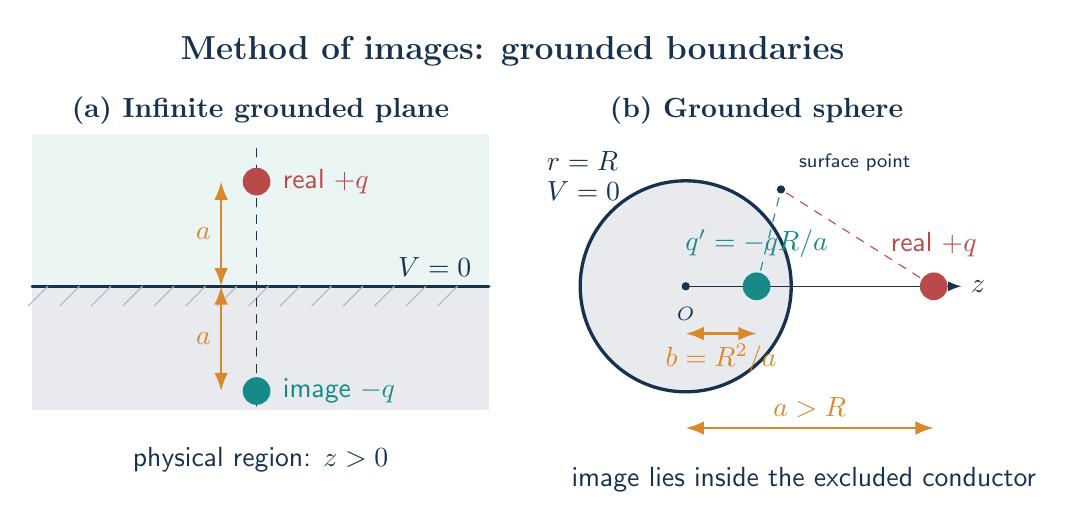
\begin{tikzpicture}[font=\sffamily,>=Latex,line cap=round,line join=round]
  \node[font=\bfseries\large,ink] at (6.2,5.0) {Method of images: grounded boundaries};

  % Grounded plane
  \begin{scope}[shift={(0.15,0)}]
    \node[font=\bfseries,ink] at (2.85,4.25) {(a) Infinite grounded plane};
    \fill[soft] (-.05,2.02) rectangle (5.75,3.95);
    \fill[ink!10] (-.05,.45) rectangle (5.75,2.02);
    \draw[ink,very thick] (-.05,2.02)--(5.75,2.02);
    \node[ink,above left] at (5.65,2.02) {$V=0$};
    \foreach \x in {.15,.55,...,5.55}\draw[ink!35] (\x,2.02)--++(-.25,-.25);
    \draw[dashed,ink] (2.8,.5)--(2.8,3.85);
    \fill[redq] (2.8,3.35) circle (5pt) node[right=6pt,redq] {real \(+q\)};
    \fill[teal] (2.8,.69) circle (5pt) node[right=6pt,teal] {image \(-q\)};
    \draw[<->,gold,thick] (2.35,2.02)--(2.35,3.35) node[midway,left] {$a$};
    \draw[<->,gold,thick] (2.35,.69)--(2.35,2.02) node[midway,left] {$a$};
    \node[ink,align=center] at (2.85,-.18) {physical region: \(z>0\)};
  \end{scope}

  % Grounded sphere
  \begin{scope}[shift={(6.55,0)}]
    \node[font=\bfseries,ink] at (2.75,4.25) {(b) Grounded sphere};
    \fill[ink!10] (1.85,2.02) circle (1.34);
    \draw[ink,very thick] (1.85,2.02) circle (1.34);
    \node[ink,align=left] at (.55,3.42) {$r=R$\\[-1pt]$V=0$};
    \fill[ink] (1.85,2.02) circle (1.5pt) node[below=4pt] {\scriptsize\(O\)};
    \draw[ink,->] (1.85,2.02)--(5.35,2.02) node[right] {$z$};
    \fill[teal] (2.75,2.02) circle (5pt) node[above=7pt,teal] {$q'=-qR/a$};
    \fill[redq] (5.0,2.02) circle (5pt) node[above=7pt,redq] {real \(+q\)};
    \draw[<->,gold,thick] (1.85,1.42)--(2.75,1.42) node[midway,below] {$b=R^2/a$};
    \draw[<->,gold,thick] (1.85,.22)--(5.0,.22) node[midway,above] {$a>R$};
    \draw[dashed,teal] (2.75,2.02)--(3.06,3.25);
    \draw[dashed,redq] (5.0,2.02)--(3.06,3.25);
    \fill[ink] (3.06,3.25) circle (1.5pt) node[above right=3pt] {\scriptsize surface point};
    \node[ink,align=center] at (3.35,-.43) {image lies inside the excluded conductor};
  \end{scope}
\end{tikzpicture}
\end{document}
